\documentclass[document.tex]{subfiles} 
\begin{document}

\chapter{مقدمة عن أنظمة التشغيل}
\textbf{جهاز الحاسب} هو مجموعة من الشرائح الإلكترونية والعتاديات والمتحكمات المرتبطة مع بعضها لتوفير منصة تشغيلية للبرامج و التي بدونها لن يعمل هذا الجهاز. ويمكن تقسيم البرامج بحسب طبيعة عملها ووظيفتها الى قسمين هما \textbf{برامج المستخدم} والتي صممت خصيصاً لحل مشاكل المستخدم و \textbf{برامج النظام} والتي تتحكم في عتاد وموارد الحاسب ، ويعتبر نظام التشغيل مثالا لبرامج النظام حيث يدير عتاد وموارد الحاسب بالإضافة الى ميزة مهمة وهي توفر بيئة تشغيل وهمية (\en{Virtual Machine}) لبرامج المستخدم.  

ويوضح التعريف السابق عدداً من المفاهيم التي يجب الوقوف عليها وتوضحيها بشكل مفصل. فجهاز الحاسب هو \textbf{منصة تشغيلية} حقيقية للأوامر ويأتي ذلك بسبب وجود متحكم خاص لمعالجة الأوامر وتنفيذها ، هذا المتحكم هو المعالج (\en{Processor}) حيث يعمل على تنفيذ الأوامر (من عمليات حسابية ومنطقية) وإرسال النتائج الى الأماكن المطلوبة. وتسمى مجموعة الأوامر التي ينفذها المعالج باسم \textbf{البرامج}، وبسبب تكلفة بناء المعالج فانه غالباً ما يتعرف على عدداً معينا من الأوامر والتي تعرف بمجموعة الأوامر (\en{Instruction Set}). لذلك حتى يتم تنفيذ أوامر أي برنامج فانها يجب أن تُكتب وفقا لمجموعة الأوامر التي يدعمها المعالج\footnote{سنتحدث عن معالجات انتل 32 بت في هذا البحث نظراً لأنها الأكثر انتشاراً.}.والشكل  \ref{fig:instruction_format} يوضح نموذجاً عاما لتعليمات وأوامر المعالج التي تتكون منها البرامج. وجزءا منها هي اختيارية وسنركز هنا على ال \en{OPCODE} والتي تمثل أوامر المعالج. 

\begin{figure}[h!] 
  \caption{الشكل العام لأوامر المعالج \en{x86}}
  \centering
   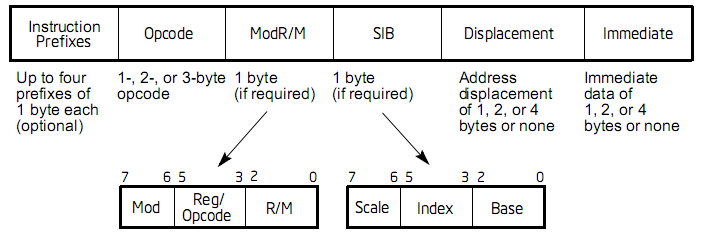
\includegraphics[width=0.7\textwidth]{../img/instruction_format}
 \label{fig:instruction_format} 
\end{figure}
 
وتشكل أوامر المعالج لغة برمجية من خلالها يمكن برمجة الحاسب وكتابة البرامج لحل مشاكل المستخدم ، هذه اللغة تسمى بلغة الآلة (\en{Machine Language}) . وتتكون هذه اللغة من الرموز \en{0} و \en{1} حيث أن أوامر المعالج ما هي الا سلسلة معينة من هذه الرموز. فمثلا لتعيين القيمة \en{31744} للمسجل \en{AX}\footnote{المسجلات هي ذواكر بداخل المعالج.} يجب أن يحوي البرنامج على الأمر \en{101110001100000000000111}. وبالتالي تكون عملية كتابة برنامج متكامل بهذه اللغة أمراً في غاية الصعوبة وكذلك مهمة تنقيح البرنامج وتطويره في المستقبل هي معقدة أيضا. لذلك ظهرت لغة التجميع لحل هذه المشكلة حيث أن اللغة تدعم مسميات ومختصرات للمسجلات ولأوامر المعالج ، فمثلا الأمر السابق في لغة التجميع يكون بالصورة التالية. 
\begin{english}
\fontspec[Scale=0.9]{Courier New}

\lstset{numberstyle=\tiny,numbers=left,stepnumber=1,numbersep=5pt,tabsize=2,extendedchars=true,breaklines=true,frame=b,showspaces=false, showtabs=false,xleftmargin=10pt,framexleftmargin=10pt,framexrightmargin=5pt,framexbottommargin=4pt,showstringspaces=false,language=[x86masm]Assembler}


\begin{lstlisting}[label=lst:mov,caption=\en{Assembly Language}]
	MOV AX,0x7C00	; Instead of 101110001100000000000111
\end{lstlisting}
\end{english}

والذي يجب تحويله الى لغة الآلة حتى يتمكن المعالج من تنفيذه ، هذا المحول يسمى \textbf{بالمجمع} والذي يقوم بتحويل أمر لغة التجميع الى ما يقابله بلغة الآلة\footnote{كل أمر بلغة التجميع يقابله أمراً واحداً بلغة الآلة لذلك حقيقة لا يوجد فرقاً في أداء البرامج المكتوبة بأي منهم ولا في حجم الملف الناتج ، وإنما يظهر الفرق في سهولة تطوير البرامج بلغة التجميع ولكن على حساب أنه يجب تحويلها عن طريق المجمع.}. ولم تنجح لغة التجميع في توفير لغة عالية المستوى تبسط عملية برمجة البرامج بشكل أكبر وذلك بسبب أنها مختصرات للغة الآلة لذلك سرعان ما تم تطوير لغات عالية المستوى مثل لغة السي\footnote{تم تطوير لغة السي بهدف برمجة نظام يونيكس \en{Unix} في معامل بيل.} والسي++ بحيث تكتب البرامج فيها بشكل مبسط بعيداً عن تعقيدات الآلة وأوامرها ومسجلاتها وتدعم هذه اللغات عددا من التراكيب وجمل التحكم العالية المستوى. ولكي ينفذ المعالج برامج هذه اللغات فانه يجب أولا ترجمة الشفرة المصدرية الى ما يقابلها بلغة التجميع وهذا يتم عن طريق برنامج يسمى \textbf{المترجم (\en{Compiler})} وبعدها يقوم المجمع بتحويل شفرة التجميع الى برنامجاً بلغة الآلة والذي يستطيع المعالج تنفيذه.   

\setlength{\fboxrule}{0pt}
   \fbox{\colorbox{light-gray}{
         \begin{minipage}[t]{0.9\textwidth} 
\Square بخصوص تمثيل البيانات والبرامج في الحاسب فإنها تمثل بطرق مختلفة تختلف على حسب وحدة التخزين و لكنها في الآخر تستخدم المنطق الثنائي وهو وجود طاقة كهربائية أم لا ، فمثلا تتكون الذاكرة الرئيسية \en{DRAM} من ملايين المكثفات (\en{Capacitors}) والترانزستورات (\en{Transistors}) لتكوين خلايا الذاكرة (\en{Memory Cells}) ، و تتكون كل خلية (والتي تشكل بت واحد من الذاكرة) من مكثف وترانزستور بحيث يحفظ المكثف قيمة الخلية (البت) والتي هي إما وجود إلكترون (منطقيا تساوي \en{1}) وإما عدمها (منطقيا تساوي \en{0}) ويعمل الترانزستور على تغيير قيمة المكثف . وعلى هذا الشكل تحفظ جميع الأوامر والبرامج في الذاكرة الرئيسية ويأتي دور المعالج لتنفيذ هذه الأوامر حيث يقوم بقرائتها وفهم وظيفتها (\en{Decode}) وتنفيذها ومن ثم يقوم بحفظ النتائج. ولكي ينفذ المعالج أي برنامج فان البرنامج يجب أن يتواجد على الذاكرة الرئيسية وليس على أحد الذواكر الثانوية (مثل القرص الصلب).
         \end{minipage}
      }
   }\\

حتى الان لم نذكر وظيفة نظام التشغيل لأن بيئة التشغيل الحقيقية هي المعالج وليست نظام التشغيل أو غيره من البرامج وعلى المبرمج الإلمام بكيفية برمجة عتاد ومتحكمات الحاسب وكيفية طباعة المخرجات على الشاشة وقراءة البيانات من متحكم لوحة المفاتيح ولا يقتصر على ذلك بل على المبرمج توفير طرقا ودوالاً لإدارة الذاكرة من حجز المقاطع وتحريرها وكذلك إدارة جميع عتاد الحاسب. كل ذلك يجعل عملية كتابة البرامج مستحيلة وهذا ما أدى الى ظهور طبقة برمجية (\en{Layer}) تدير عتاد وموارد الحاسب وتوفر واجهة برمجية للمبرمج لكي يتعامل مع هذه الموارد.هذه الطبقة سميت \textbf{بنظام التشغيل (\en{Operating System})}. الهدف الرئيسي لهذه الطبقة هي عزل المبرمج عن تعقيدات العتاد بحيث أن إدارة هذه العتاديات أصبحت من مهمة هذه الطبقة وفي نفس الوقت توفر واجهة برمجية (أو جهاز تخيلي) للإستفادة من هذه العتاديات. والشكل \ref{fig:computer_layer} يوضح موضع هذه الطبقة (نظام التشغيل) في حالة قسمنا جهاز الحاسب الى عدة طبقات \cite{2}.
\begin{figure}[h!] 
  \caption{طبقات الحاسب}
  \centering
   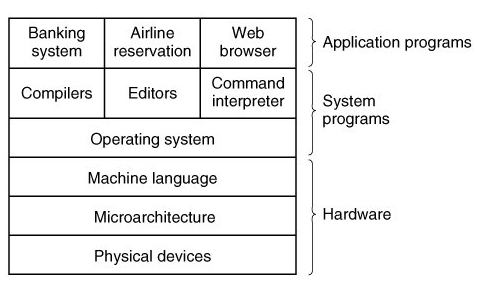
\includegraphics[width=0.7\textwidth]{../img/computer_layer}
 \label{fig:computer_layer} 
\end{figure}
وأدنى طبقة هي طبقة العتاديات (\en{Device Level}) حيث تتكون من المتحكمات ومن الشرائح المتكاملة (\en{Integrated Circuit}) والأسلاك وكل ما يتعلق بالأجهزة المادية.يلي هذه الطبقة طبقة \en{Microarchitecure} وفيها تظهر بريمجات (\en{Mircoprogram}) تتحكم في عمل المتحكمات لكي تؤدي وظيفتها فمثلاً بريمج ال \en{data path} بداخل المعالج والذي يقوم في كل دورة للساعة (\en{Clock Cycle}) بجلب قيمتين من المسجلات الى وحدة الحساب والمنطق (\en{Arithmetic Logic Unit}) التي تجري عليهم عملية ما ومن ثم تقوم بحفظ النتيجة في أحد المسجلات. وظيفة \en{data path} هي تنفيذ الأوامر والتعليمات وذلك بارسالها الى وحدة الحساب والمنطق ، وتشكل مجموعة الأوامر المدعومة وكذلك المسجلات المرئية لمبرمج لغة التجميع طبقة مجموعة الأوامر (\en{Instruction Set Architecture}) وتسمى هذه الطبقة طبقة الآلة (\en{Machine Language}) حيث تحوي على كل الأوامر التي يدعمها المعالج بما فيها أوامر القراءة والكتابة من مسجلات متحكمات العتاد (\en{Device Controller}) . ويلي هذه الطبقة طبقة نظام التشغيل والتي تفصل وتعزل العتاد عن المستخدم فبدلاً من أن يقوم المبرمج ببرمجة متحكم القرص الصلب ونظام للملفات حتى يتمكن من قراءة ملف على القرص فان النظام يوفر واجهة مبسطة  بالصورة \cmd{read(fd,buffer,size)}. وأخيراً توجد طبقة البرامج (برامج النظام والمستخدم)  ولا تصنف الكثير من برامج النظام ضمن نظام التشغيل حيث أن البرامج التي تتبع لنظام التشغيل يجب أن تعمل في مستوى النواة (\en{Kernel Mode}) وليس في المستويات الأخرى\footnote{في الفصل الثاني بإذن الله سيتم الحديث عن مستويات الحماية في المعالجات.}.  


\section{ما هو نظام التشغيل}
من الصعب إيجاد تعريفاً واضحاً لأنظمة التشغيل فما يعتبره البعض تابعاً لنظام ما لا يعتبره الآخرون كذلك. لكن ما تم الإتفاق عليه هو أن\textbf{ نظام التشغيل} يدير عتاد وموارد الحاسب ويوفر واجهة برمجية (جهاز تخيلي) من خلالها يمكن الإستفادة من هذه الموارد. 
\subsection{نظام التشغيل كجهاز تخيلي }
مما سبق نجد أن الواجهة التي تقدمها طبقة الآلة (\en{Machine Language Level}) هي بدائية ويصعب استخدامها في كتابة البرامج ، فكما ذكرنا كمثال للقراءة من ملف على القرص يجب أن يحوي البرنامج على شفرة لنظام الملفات حتى نعرف عنوان الملف الفيزيائي على القرص، وكذلك يجب أن يحوي البرنامج على شفرة للتعامل مع متحكم القرص الصلب وهي شفرة ليست باليسيرة حيث للقراءة من القرص يجب تحديد رقم المقطع ورقم الرأس ورقم المسار وتحديد الذاكرة المؤقتة (\en{Buffer}) حتى يتم تحميل المقاطع اليها.كل هذه الأمور لو استمرت بهذا الشكل لما وصلت التطبيقات لما هي عليها الان، لذلك كان الحل هو بإيجاد طبقة نظام التشغيل والتي توفر واجهة أو أوامر مبسطة ومجردة من تفاصيل وتعقيدات العتاد لكي تستخدمها البرامج بدلا من الأوامر التي توفرها طبقة الآلة .

\subsection{نظام التشغيل كمدير للموارد والعتاد}
بعد أن تم عزل المبرمج بواسطة طبقة نظام التشغيل فان هذه الطبقة تقدم بجانب الواجهة البرمجية إدارة لعتاد الحاسب (المعالج،الذاكرة،الأقراص الصلبة والمرنة،كرت الشبكة،وغيرها من المتحكمات) ، ومهمة إدارة العتاد تتركز في حجز العتاد وتحريره ، فمثلاً يقوم نظام التشغيل بإدارة المعالج نفسه وذلك بأن يحجز المعالج لبرنامج ما ومن ثم يحرر المعالج ويحجزه لبرنامج آخر (تعدد المهام \en{Multitasking}) وكذلك يدير النظام أهم موارد الحاسب وهي الذاكرة الرئيسية وذلك بحجز مقاطع من الذاكرة (\en{Memory Blocks}) بناءاً على طلب برامج المستخدم وكذلك عملية تحرير الذواكر وإدارة الذاكرة التخيلية ومفهوم الصفحات. 

\section{تاريخ أنظمة التشغيل}
خلال سنوات مضت تطورت أنظمة التشغيل تطوراً ملحوظاً من أنظمة تشغيل لبرنامجاً واحدا الى أنظمة موزعة تسمح بتشغيل أكثر من برنامج على عدة حواسيب مختلفة. هذا التطور سببه الرئيسي تطور الحاسبات والمعالجات وازدياد حجم الذواكر بشكل رهيب. وفي هذا الجزء سنلقي نظرة على تطور أجيال الحواسيب وبعض أنظمة التشغيل التي استخدمت في تلك الفترات.
 
\subsection{الجيل الصفري (1624-1945): الحواسيب الميكانيكية}
أول محاولة لبناء آلة حسابية كانت من قبل العالم الفرنسي بليز باسكال\footnote{والذي تم تسمية لغة البرمجة باسكال باسمه تشريفاً له.} في عام 1642 عندما كان عمره 19 عاماً وذلك لمساعدة والده الذي كان يعمل محصلاُ للضرائب لمصلحة الحكومة الفرنسية.هذه الآلة (وتعرف بالاسم \en{Pascaline}) هي ميكانيكية بالكامل وتوفر فقط عملية الجمع والطرح (انظر الشكل \ref{fig:Pascaline}).

\begin{figure}[h!] 
  \caption{آلة باسكال}
  \centering
   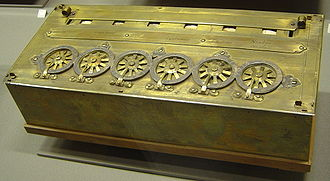
\includegraphics[width=0.5\textwidth]{../img/Pascaline}
 \label{fig:Pascaline} 
\end{figure}

وبعد حوالي 30 عاماً قام العالم الرياضي جوتفريد ليبنز \en{Gottfried Wilhelm Leibniz} ببناء آلة حسابية ميكانيكية أخرى (تم الإنتهاء منها في عام 1694 وسميت بالاسم \en{Step Reckoner}) ولكن هذه المرة أصبح من الممكن إجراء العمليات الحسابية الأربعة: الجمع والطرح و الضرب والقسمة (الشكل \ref{fig:Leibnitzrechenmaschine}).
\begin{figure}[h!] 
  \caption{آلة  \en{Step Reckoner} في متحف بألمانيا}
  \centering
   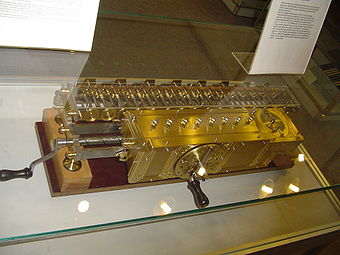
\includegraphics[width=0.5\textwidth]{../img/Leibnitzrechenmaschine}
 \label{fig:Leibnitzrechenmaschine} 
\end{figure}
 ومضت حوالي 150 عاماً بدون أي شيء يذكر حتى قام البروفيسور شارلز بابباج \en{Charles Babbage} بتصميم آلة محرك الفروق \en{Difference engine} (انظر الشكل \ref{fig:DifferenceEngine}) ، وهي آلة ميكانيكية أيضا تشابه آلة باسكال في أنها لا توفر سوى عمليتي الجمع والطرح لكن هذه الآلة تم تصميمها لغرض حساب قيم دوال كثيرات الحدود باستخدام طرق التقريب المنتهية (\en{Method of Finite Differences}) .
\begin{figure}[h!] 
  \caption{محرك الفروق بعد أن قام ابن بابباج بتجميعه}
  \centering
   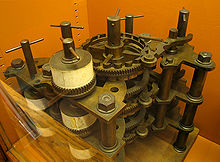
\includegraphics[width=0.5\textwidth]{../img/BabbageDifferenceEngine}
 \label{fig:DifferenceEngine} 
\end{figure}
وما ميز هذه الآلة هي طريقة إخراج النتائج حيث تنقش النتائج على ألواح نحاسية. وعلى الرغم من أن آلة الفروق عملت جيداً إلا أن تصميمها كان يسمح بحساب خوارزمية واحدة فقط\footnote{في عام 1991 قام متحف العلوم بلندن ببناء نموذج مكتمل لمحرك الفروق.} وهذا ما جعل شارلز بابباج يعيد محاولته مجدداً ويستهلك جزءاً ضخما من وقته ومن ثروة حكومته في بناء آلة أخرى عٌرفت بالمحرك التحليلي \en{Analytical Engine} (انظر الشكل \ref{fig:AnalyticalMachine}). هذا المحرك (وهو أيضا آلة ميكانيكية بالكامل) احتوى على أربع مكونات: المخزن (الذاكرة \en{Memory})، الطاحنة (وحدة الحساب \en{Computation Unit}) ، وحدة الإدخال (قارئ البطاقات المثقبة \en{Punched Card Reader}) ووحدة الإخراج (البطاقات المثقبة واللوحات المطبوعة).  ويتكون المخزن من 1000 كلمة (\en{Word}) بطول 50 رقم صحيح وتستخدم لحفظ المتغيرات والنتائج ، أما الطاحنة فتستقبل الوسائط من المخزن وتجري عليهم أي من العمليات الرياضية الأربعة ومن ثم تحفظ النتائج في المخزن.
الميزة الأساسية للمحرك التحليلي هو قدرته على حل عدد كبير من المشاكل (على عكس محرك الفروق) حيث تكتب البرامج في بطاقات مثقبة ويتم قرائتها الى المحرك بواسطة قارئاً لهذه البطاقات. وتحوي هذه البطاقات على أوامر موجه الى المحرك لكي يقوم بقرائة عددين من المخزن ويجري عملية ما (جمع مثلا) ومن ثم يحفظ النتيجة في المخزن أيضا ، وكذلك تحوي أوامر أخرى مثل المقارنة بين عددين والتفرع ونقل التنفيذ. ولأن المحرك قابل للبرمجة (بلغة شبيهة بلغة التجميع) فقد استعان شارلز بابباج بالمبرمجة آدا لوفلاس \en{Ada Lovelace} والتي صنفت كأول مبرمج في التاريخ. ولسوء الحظ لم ينجح شارلز بابباج في أن يزيد من دقة المحرك ربما لأنه يحتاج الى آلافاً من التروس والعجلات. وبشكل أو بآخر يعتبر شارلز باباج الجد الأول للحواسيب الحالية حيث أن فكرة عمل المحرك التحليلي مشابهة للحواسيب الحالية.

\begin{figure}[h!] 
  \caption{المحرك التحليلي بمتحف في لندن}
  \centering
   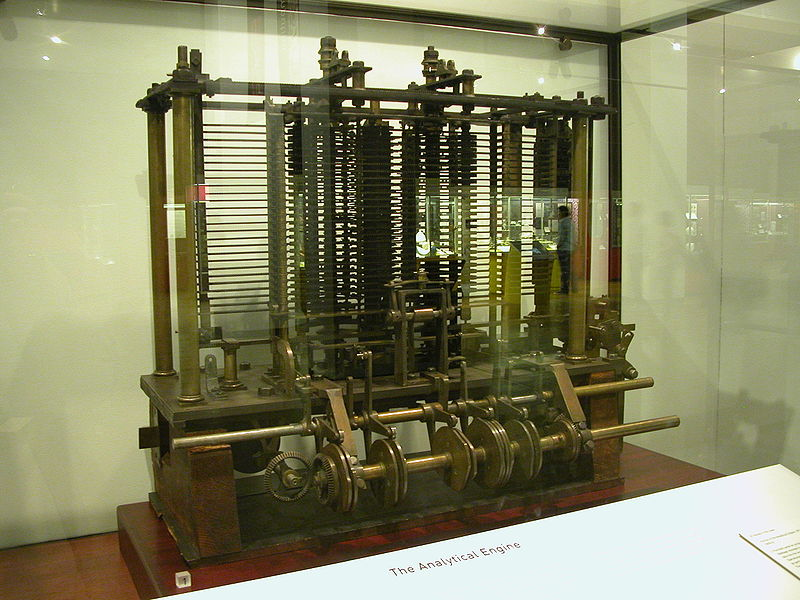
\includegraphics[width=0.5\textwidth]{../img/AnalyticalMachine}
 \label{fig:AnalyticalMachine} 
\end{figure}
وفي أواخر 1930 قام الطالب الألماني كونارت تسوزا \en{Konrad Zuse} ببناء آلة حسابية ولكنها تعتمد على الريلاي (\en{Relay}) وسميت بجهاز \en{Z1} (انظر الشكل \ref{fig:Z1}) وتعتبر أول حاسبة تعتمد على الريلاي وعلى المنطق الثنائي في عملها. ولسوء الحظ تم تدمير الحاسبة \en{Z1} في انفجار في برلين أثناء الحرب العالمية الثانية عام 1943. وعلى الرغم من أن تصميم \en{Z1} لم يؤثر في تصاميم الحواسيب التي تليه بسبب تدميره هو وجميع خطط بنائه إلا أنه يعتبر أحد التصاميم التي كان لها أثرها ذاك الوقت.
\begin{figure}[h!] 
  \caption{حاسبة \en{Z1} بعد إعادة انشائها في متحف بألمانيا}
  \centering
   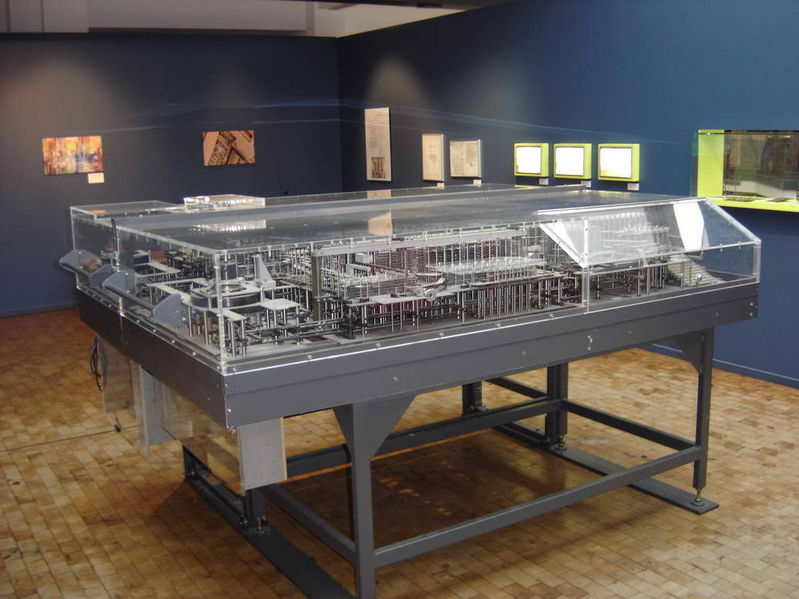
\includegraphics[width=0.5\textwidth]{../img/Z1}
 \label{fig:Z1} 
\end{figure}
وبعد برهة من الزمن قام جون أتاناسوف \en{John Vincent Atanasoff} بتصميم جهاز \en{Atanasoff}(انظر الشكل \ref{Atanasoff-Berry}) والذي كان مدهشا في وقته حيث يستخدم التحسيب الثنائي (\en{Binray Arithmetic}) ويحوي مكثفات للذاكرة ولكن الجهاز لم يكن عمليا.
\begin{figure}[h!] 
  \caption{حاسبة \en{Atanasoff} بعد إعادة انشائها في جامعة \en{Iowa State}}
  \centering
   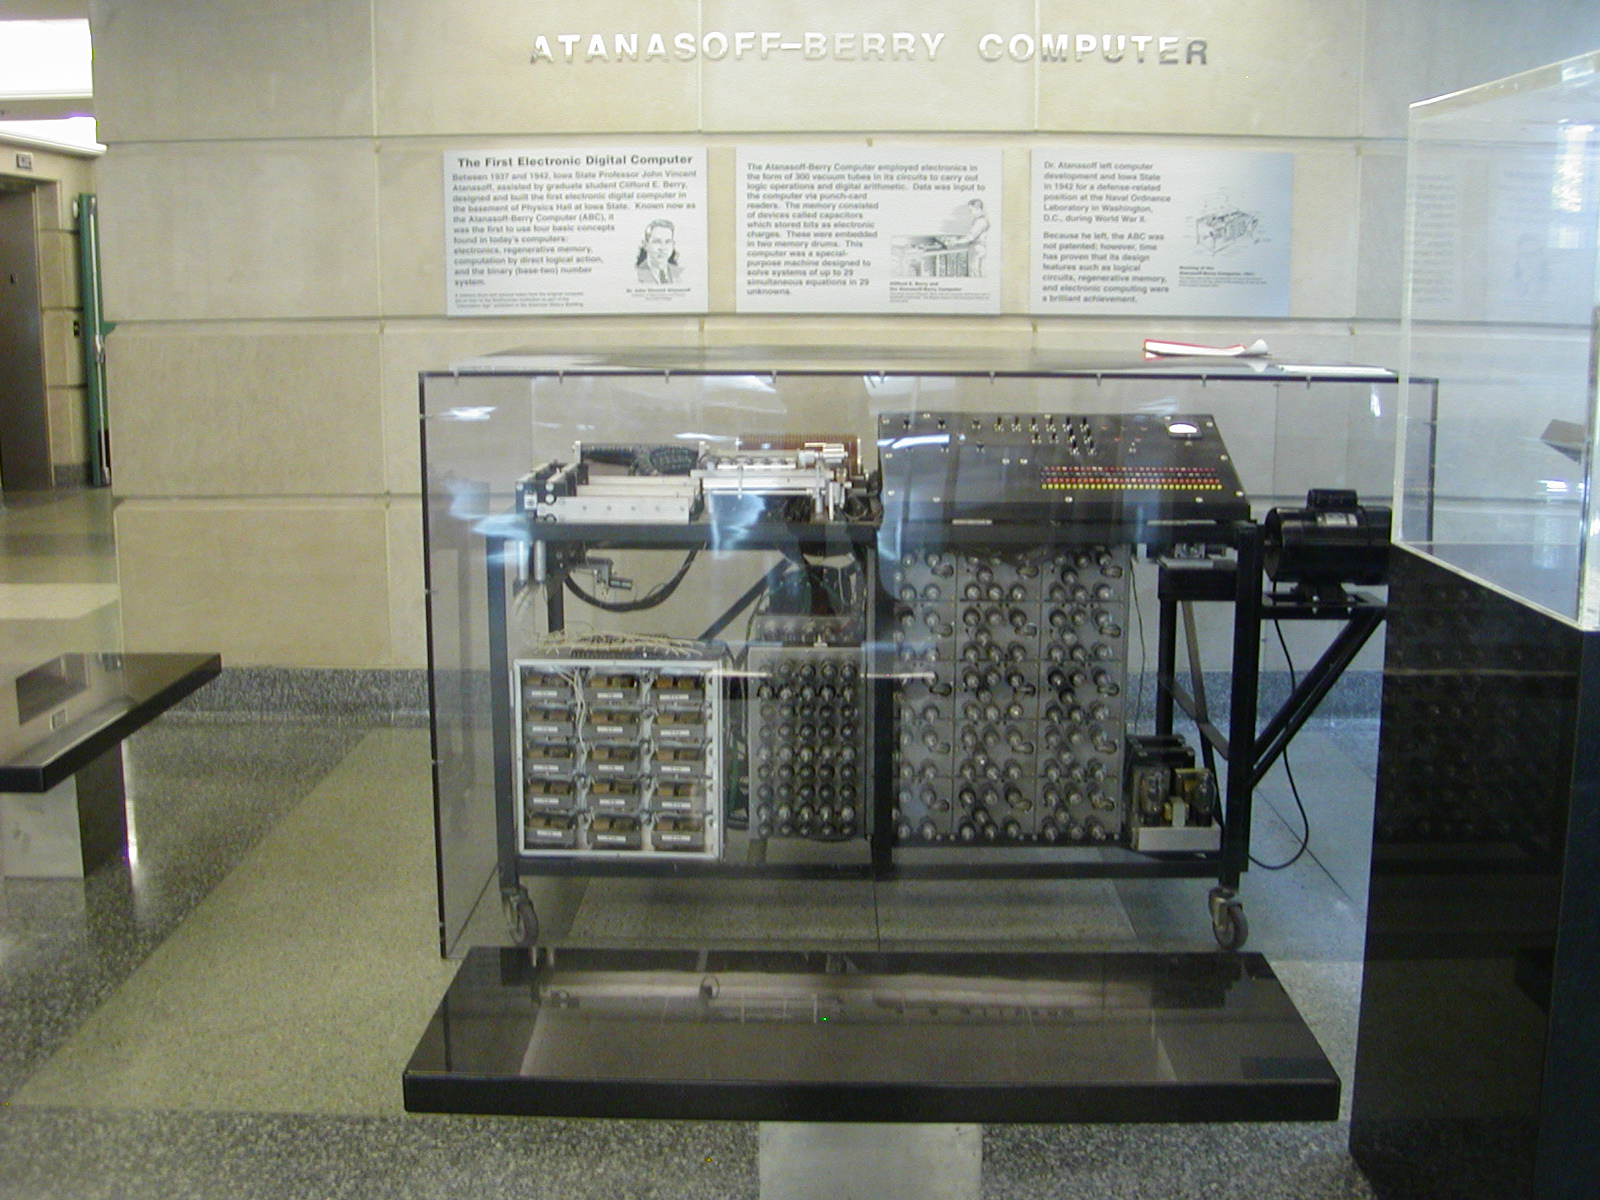
\includegraphics[width=0.5\textwidth]{../img/Atanasoff-Berry}
 \label{fig:Atanasoff-Berry} 
\end{figure}
وفي بدايات 1940 قام هوارد ايكين \en{Howard Aiken} بتصميم الحاسبة \en{ASCC} - والتي أعيد تسميتها الى \en{Harvard Mark I} - في جامعة هافارد (انظر الشكل \ref{fig:HarvardMarkI}).وقد أتبع هوارد نفس منهج بابباج وقرر أن يعتمد على الريلاي وأن يصمم حاسبة للأغراض العامة والتي فشل بها شارلز بابباج.وفي عام 1944 تم الإنتهاء من تصميمها وتم تصميم نسخة محسنة أيضا سميت ب \en{Harvard Mark II}.ومع هذا التصميم انتهى عصر الحاسبات الميكانيكية والريلاي وبدأ عصر جديد.
 
\begin{figure}
  \centering
  \subfloat[الجزء الأيسر من حاسبة \en{Mark I}]{\label{fig:MarkILeftSegment}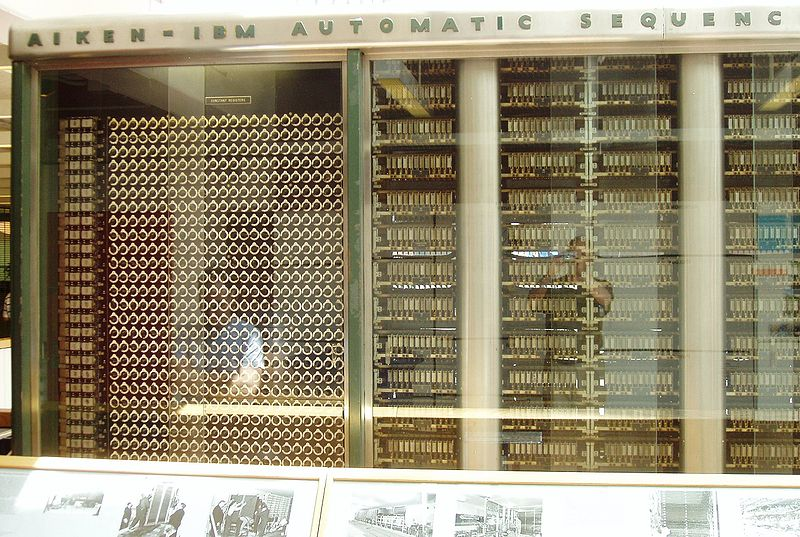
\includegraphics[width=0.5\textwidth]{../img/MarkILeftSegment}}                
 \subfloat[الإدخال والإخراج والتحكم]{\label{fig:MarkInput-OutputDetails
}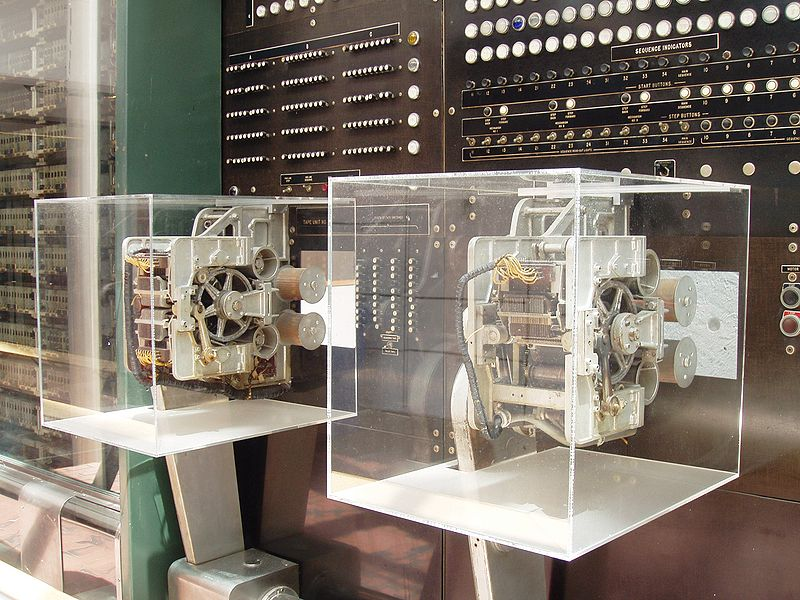
\includegraphics[width=0.4\textwidth]{../img/MarkInput-OutputDetails}}
  \caption{حاسبة \en{Harvard Mark I}}
  \label{fig:HarvardMarkI}
\end{figure}

\subsection{الجيل الأول (1945-1955): الصمامات المفرغة و لوحات التوصيل}
في بدايات الحرب العالمية الثانية ، كان أمير البحرية في برلين يرسل رسائل الى الغواصات الألمانية عبر موجات الراديو والتي استطاع حلفاؤها البريطانيين التقاطها ، ولسوء حظهم كانت الرسائل ترسل مشفرة وذلك عن طريق شفرة خاصة تنتج من قبل جهاز يسمى بجهاز إنجما (\en{Enigma Machine} والذي تم تصنيعه لتشفير الرسائل وفك تشفيرها .
\begin{figure}[h!] 
  \caption{آلة إنجما الألمانية لتشفير الرسائل وفكها}
  \centering
   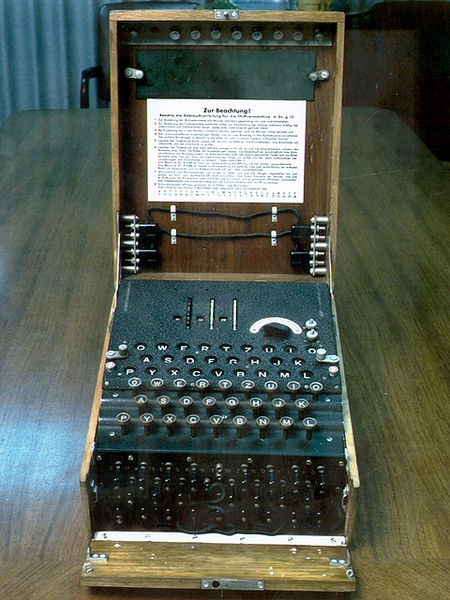
\includegraphics[width=0.5\textwidth]{../img/Enigma}
 \label{fig:Enigma} 
\end{figure}
 وقد تمكنت الإستخبارات البريطانية من الحصول على أحد هذه الأجهزة وذلك بعد الإتفاق مع الإستخبارات البولندية والتي كانت قد سرقت جهازاً من الألمان.  وحتى يتمكن البريطانيين من فك شفرة الرسائل فان هذا يتطلب وقتاً وعمليات حسابية طويلة ، لذلك سرعان ما أسست معملا سريا يحوي على حاسبة الكترونية عرفت بالاسم \en{Colossus}. هذه الحاسبة تم تصميمها من قبل عدة أشخاص وشارك فيها العالم آلان تورنج وأصبحت جاهزة للعمل في عام 1943.  وبسبب كون المشروع سريا وتم التكتم عليه لما يقارب 30 عاما فان هذا النوع من الحواسيب لم يؤثر على تصاميم الحواسيب الحديثة ولكن يجدر بالذكر أن هذه الحاسبة تعتبر أول حاسبة إلكترونية قابلة للبرمجة تستخدم الصمامات الهوائية في حساباتها. 

\begin{figure}[h!] 
  \caption{الحاسبة \en{colossus} التي كسرت شفرة إنجما}
  \centering
   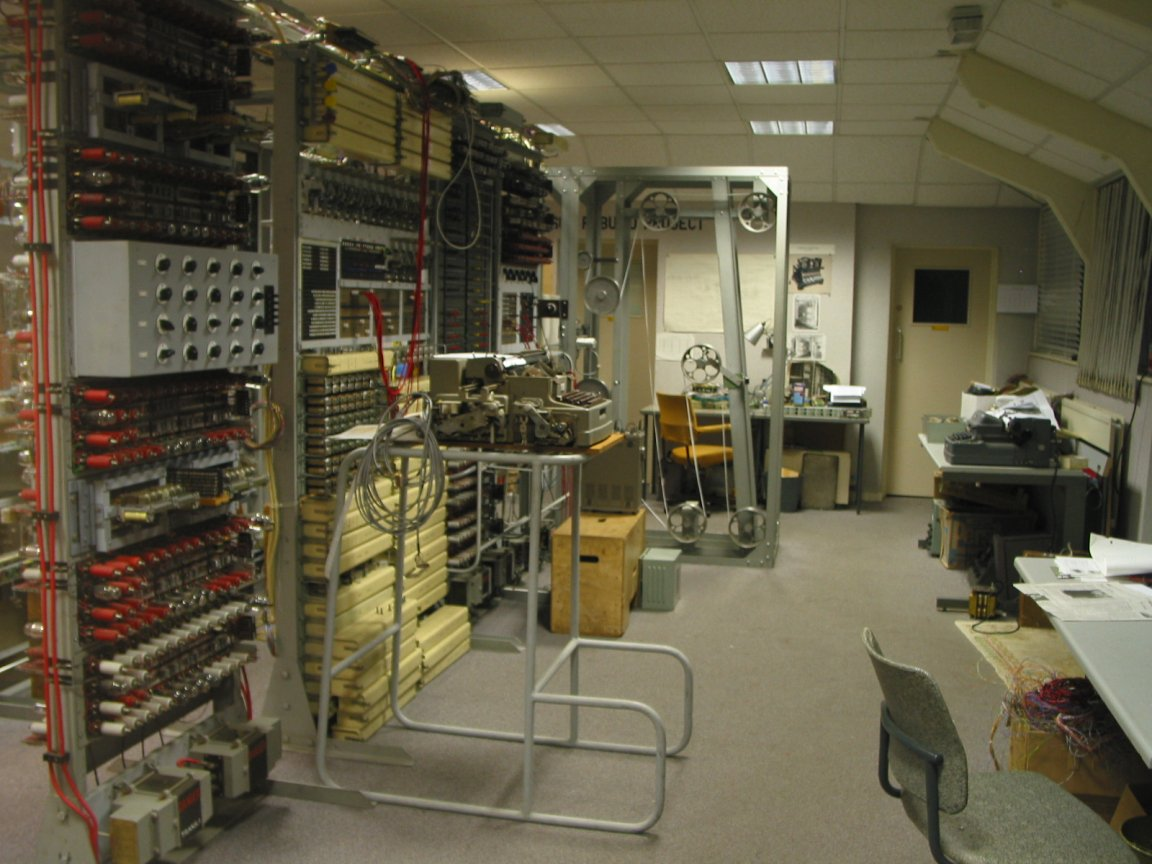
\includegraphics[width=0.5\textwidth]{../img/colossus}
 \label{fig:colossus} 
\end{figure}

وفي عام 1943 قدم جون موكلي \en{John Mauchley} مقترحاً الى الجيش الأمريكي طالباً تمويله بالمال للبدء بتصميم حاسبة إلكترونية لحساب جداول إطلاق المدفعيات بدلاً من حسابها يدويا وذلك لتقليل الأخطاء وكسب الوقت، وقد تمت الموافقة على المشروع وبدأ جون موكلي وطالبه الخريج إيكريت ببناء حاسبة تم تسميتها بالاسم إيناك \en{ENIAC} اختصارا للجملة \en{Electronic Numerical Integrator And Computer}. وتتكون من 18000 صماما مفرغا (\en{Vacuum Tubes}) و 1500 حاكمة (\en{Relays}) ، وتزن الحاسبة 30 طن وتستهلك 140 كيلو واط من الطاقة. وداخليا تحتوي الحاسبة على 20 مسجل كل منهم يسع عددا صحيحا بطول 10 خانات. وتتم برمجة إيناك عن طريق 6000 مفتاح \en{Switch}.

\begin{figure}[h!] 
  \caption{الحاسبة \en{ENIAC}}
  \centering
   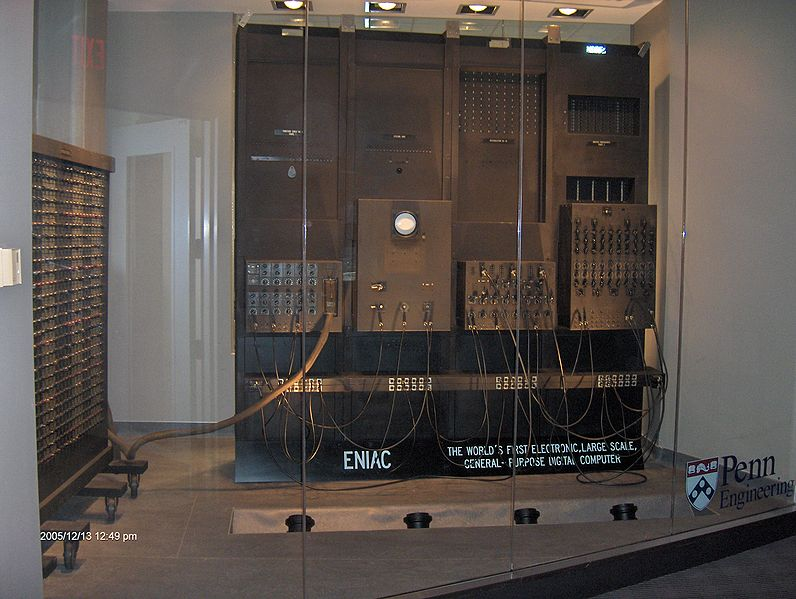
\includegraphics[width=0.5\textwidth]{../img/ENIAC}
 \label{fig:ENIAC} 
\end{figure}

وقد تم الإنتهاء من تصميم إيناك عام 1946 ، الوقت الذي كانت الحرب قد انتهت ولم تستخدم الحاسبة لهدفها الرئيسي. وبعد ذلك نظم جون موكلي وطالبه إيكريت مدرسة صيفية لوصف مشروعهم للباحثين والمهتمين. الأمر الذي أسفر عن ظهور عدد كبير من الحاسبات الضخمة . وأول حاسبة بعدها كانت \en{EDSAC} في عام 1949 بواسطة ويلكس في جامعة كامبردج. كذلك تلته الحاسبات \en{JOHNIAC} و \en{ILLIAC} وغيرهم.بعد ذلك بدأ جون موكلي وإيكريت بالعمل على حاسبة أخرى سميت بالاسم \en{EDVAC} اختصارا للجملة \en{Electronic Discrete Variable Automatic Computer} والتي كانت تعمل بالأرقام الثنائية بدلا من العشرية (كما في إيناك).بعد ذلك توقف المشروع بسبب أن جون وإيكريت قد أنشئا شركتهم الخاصة.
 
\begin{figure}[h!] 
  \caption{الحاسبة \en{EDVAC}}
  \centering
   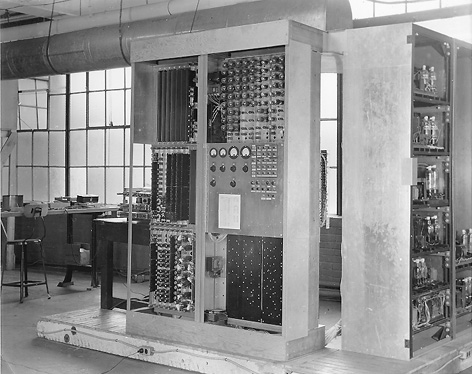
\includegraphics[width=0.5\textwidth]{../img/edvac}
 \label{fig:edvac} 
\end{figure}

%\subsection{الجيل الثاني (1955-1965): الترانزستورات}
%\subsection{الجيل الثالث (1965-1980): الدوائر المتكاملة}
%\subsection{الجيل الرابع (من 1980 حتى الان): الحواسيب الشخصية}

%\section{مكونات ومفاهيم أنظمة التشغيل}
%\section{أمثلة على أنظمة تشغيل}
%\section{نظام إقرأ}

\end{document}